% !TEX root = ../main.tex

\chapter{直流侧：CS 线圈的 1.5~kV 整流供电}
\label{chap:rect}

\section{电压变换与控制}

CS 线圈需要电压可调、电流很大的直流电源。实验一用 70~MVA、10/1.2~kV 的 $\Delta$/Y 变压器降压，六脉波全控桥整流后接时变 R-L 负载。连续电流下全控桥的平均输出为\cite{mohan2003}
\begin{equation}
V\sub{dc}=\frac{3\sqrt2}{\pi}U\sub{LL}\cos\alpha\approx1.35U\sub{LL}\cos\alpha.
\label{eq:rect}
\end{equation}
取 $U\sub{LL}=1.2$~kV、$V\sub{dc}=1.5$~kV，得初始触发角 $\alpha_0=\arccos[1500/(1.35\times1200)]=22.192^\circ$。短时仿真测得二次侧三个线电压有效值为 1199.37、1199.36、1199.22~V，最大相差 0.15~V，相序和变比正确。这一检查在接入整流桥和复杂负载之前完成，可以把电源接线问题与后级控制问题分开。

闭环控制器只看直流电压误差。式~\eqref{eq:rect} 在 $0^\circ<\alpha<90^\circ$ 内单调下降，$V\sub{dc}$ 偏低时减小 $\alpha$，反之增大。实现上以 $\alpha_0$ 作前馈工作点，PI 只补偿负载变化和模型误差，输出限制在 $5^\circ$--$80^\circ$。详细模型另加 10~ms 低通和积分限幅，避免 300~Hz 纹波直接驱动积分器。

全过程采用平均值模型：按式~\eqref{eq:rect} 产生直流电压并保留一阶变流器动态，省略器件级换相，以 0.01~s 步长跑完 460~s。六脉波详细模型只跑 0.5~s，用于验证式~\eqref{eq:rect} 背后的触发顺序和纹波机制。两层模型共用同一套负载参数和测量定义，慢动态指标和开关级波形可以直接对照。

\begin{figure}[htbp]
\centering
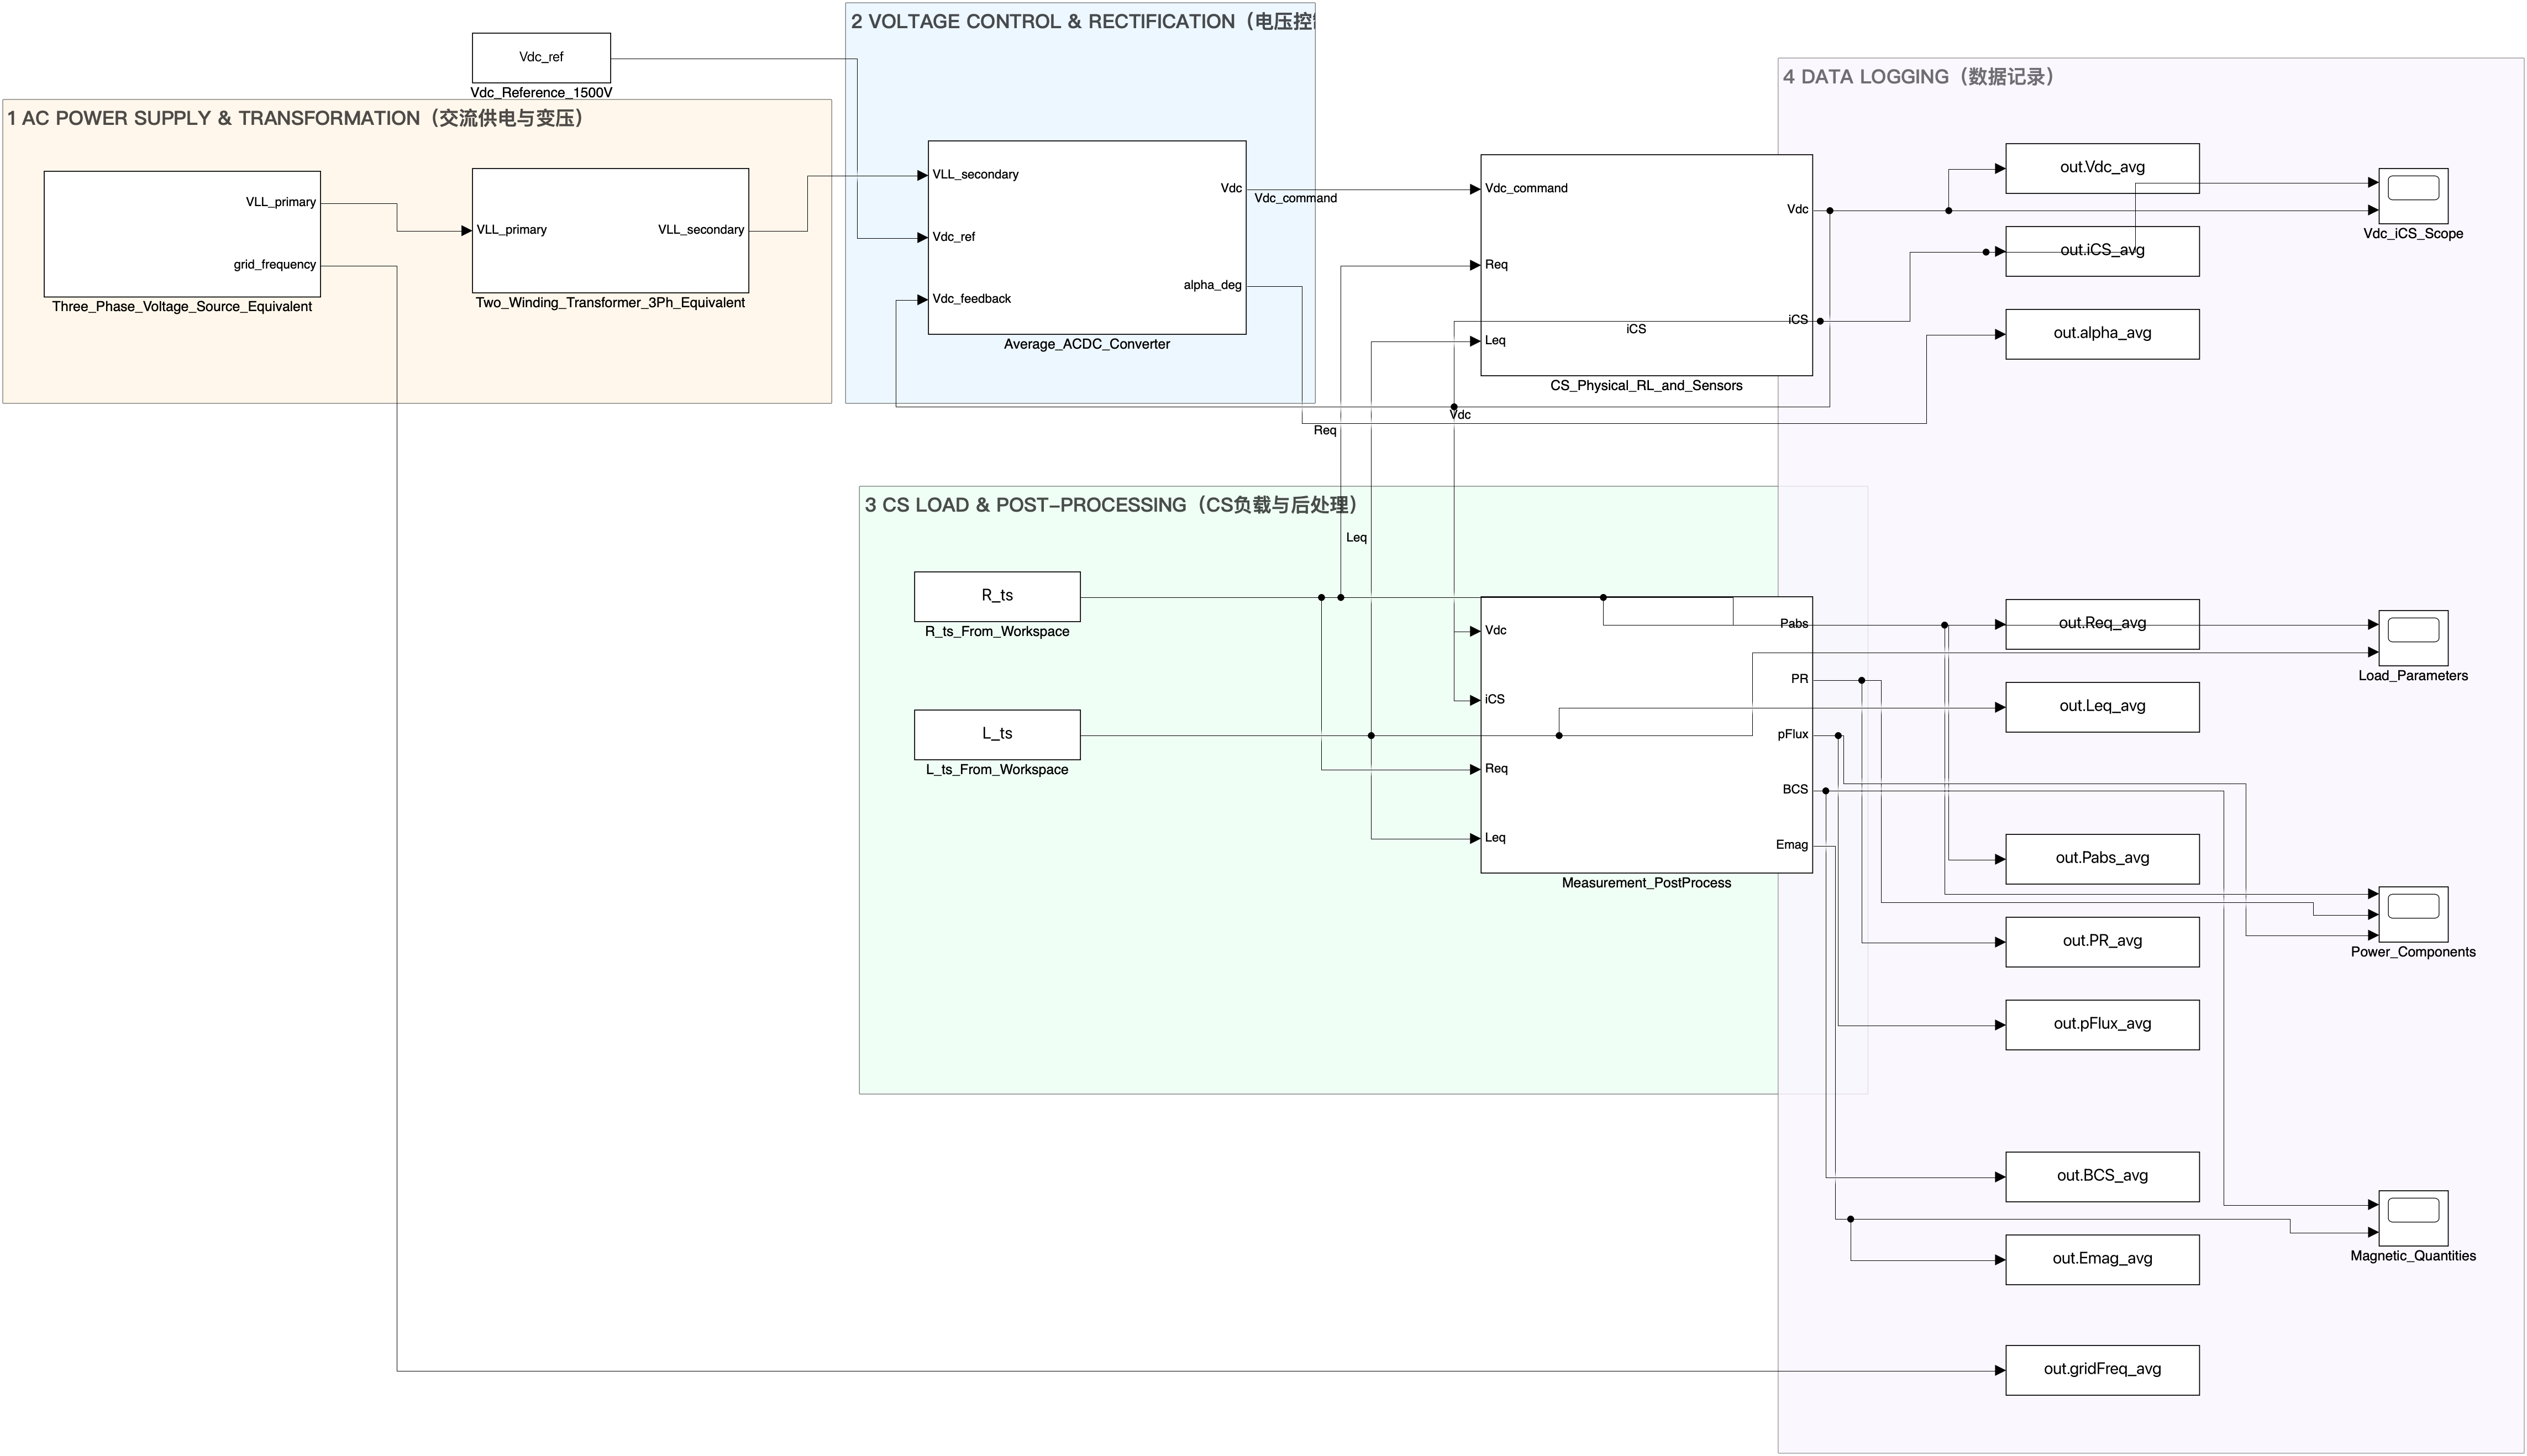
\includegraphics[width=0.66\linewidth]{native/model_cs.png}
\caption{实验一平均值模型顶层（Simulink 原生视图）：交流电源与变压、电压控制与整流、CS 负载与后处理、数据记录}
\label{fig:cs-native}
\end{figure}

\section{时变等效负载}

负载方程为
\begin{equation}
v\sub{CS}=R\sub{eq}(t)\,i\sub{CS}+\frac{\dd}{\dd t}\bigl[L\sub{eq}(t)\,i\sub{CS}\bigr].
\label{eq:cs-load}
\end{equation}
九个关键点（表~\ref{tab:cs-points}）在 0.01~s 网格上用 PCHIP 插值。选择 PCHIP 是因为它在关键点之间不产生过冲：$R\sub{eq}$ 在 12~s 附近由 0.6~$\Omega$ 降到 0.024~$\Omega$，普通样条的过冲会让电流曲线出现虚假拐点。这九个点描述的是整流器看到的等效端口，并非超导绕组本身的电阻或某一线圈的自感。Simscape 的 Variable Inductor 直接实现 $\dd(Li)/\dd t$，不需要再额外串联 $i\,\dd L/\dd t$ 电压源。

\begin{dtable}{htbp}{时变等效端口参数的九个关键点}
\label{tab:cs-points}
\begin{tabularx}{0.72\linewidth}{RRRL}
\toprule
\headrow $t$ / s & $R\sub{eq}$ / $\Omega$ & $L\sub{eq}$ / H & 阶段 \\
\midrule
0   & 0.35  & 1.10 & 预磁化 \\
5   & 0.80  & 1.08 & 击穿开始 \\
8   & 0.60  & 1.03 & 通道形成 \\
12  & 0.024 & 0.98 & 高导电形成 \\
45  & 0.024 & 0.95 & 爬升后段 \\
70  & 0.12  & 1.02 & 平顶开始 \\
335 & 0.12  & 1.00 & 平顶结束 \\
420 & 0.25  & 1.08 & 降流过程 \\
460 & 0.35  & 1.12 & 终止末段 \\
\bottomrule
\end{tabularx}
\end{dtable}

\section{全过程结果}

460~s 平均值模型的结果见图~\ref{fig:cs-overview}。直流电压全程稳定在 1.5~kV。电流可分三段：12~s 之前 1~H 量级的电感限制了电流变化率；12--45~s 电阻降到 0.024~$\Omega$，电源电压几乎全部用于建立磁链，电流快速爬升，在 50.262~s 达到峰值 39.746~kA；70~s 以后电阻回到 0.12~$\Omega$，电流朝 $1500/0.12=12.5$~kA 的平衡点衰减并形成平台，335~s 后电阻继续上升，电流降到 4.39~kA 结束。

\twofig{native/cs_voltage_current.pdf}{native/cs_power_field_energy.pdf}{平均值模型 460~s 的 MATLAB 原生波形：(a) 直流电压与 CS 电流，(b) 功率、工程磁场与磁场储能}{fig:cs-overview}

输入功率 $P\sub{abs}=v\sub{CS}i\sub{CS}$ 峰值为 59.619~MW，与电流峰值同时出现。磁场按 $B\sub{CS}=13i\sub{CS}/45000$ 换算，峰值 11.482~T。储能 $E\sub{mag}=\tfrac12L\sub{eq}i\sub{CS}^2$ 在 50.602~s 达到 0.7571~GJ，比电流峰值晚 0.34~s，原因是 $L\sub{eq}$ 此时仍在变化。

由式~\eqref{eq:cs-load} 可写出磁链相关功率及储能变化率：
\begin{equation}
p\sub{flux}=L\sub{eq}i\sub{CS}\frac{\dd i\sub{CS}}{\dd t}+i\sub{CS}^2\frac{\dd L\sub{eq}}{\dd t},\qquad
\frac{\dd E\sub{mag}}{\dd t}=L\sub{eq}i\sub{CS}\frac{\dd i\sub{CS}}{\dd t}+\frac12i\sub{CS}^2\frac{\dd L\sub{eq}}{\dd t}.
\end{equation}
两者相差 $\tfrac12i\sub{CS}^2\,\dd L\sub{eq}/\dd t$，只要电感在变，$p\sub{flux}$ 就不等于储能变化率。约 60~s 附近 $p\sub{flux}<0$，对应 $L\sub{eq}$ 减小、回路向端口释放磁能。

\section{与 ODE 基准的对比}

课程提供的 MATLAB ODE 基准保留八个时刻的电流值。表~\ref{tab:cs-ode} 中最大偏差为 0.247\%，出现在 5~s，12~s 之后基本在 0.1\% 以内，误差没有随时间累积，说明物理 R-L 网络与 ODE 基准求解的是同一方程。四项指标的最大绝对误差分别为：电流 0.247\%（5~s）、输入功率 0.147\%（8~s）、磁场 0.724\%（8~s）、储能 0.607\%（8~s）；8~s 附近百分比偏大，是因为基准值在这一带只有两位有效数字。

\begin{dtable}{htbp}{八个关键时刻的 CS 电流与 ODE 基准}
\label{tab:cs-ode}
\begin{tabularx}{0.72\linewidth}{RRRR}
\toprule
\headrow $t$ / s & 基准 / kA & 模型 / kA & 误差 / \% \\
\midrule
5   & 1.93  & 1.9252 & $-0.247$ \\
8   & 2.20  & 2.1966 & $-0.156$ \\
12  & 5.31  & 5.3149 & $+0.093$ \\
45  & 37.80 & 37.7963 & $-0.010$ \\
70  & 19.54 & 19.5443 & $+0.022$ \\
335 & 12.50 & 12.5014 & $+0.011$ \\
420 & 6.21  & 6.2056 & $-0.071$ \\
460 & 4.39  & 4.3906 & $+0.013$ \\
\bottomrule
\end{tabularx}
\end{dtable}

\section{六脉波详细模型}

图~\ref{fig:cs-detail} 是详细模型 0.20--0.24~s 窗口的波形：六路脉冲按 $60^\circ$ 电角度依次触发，每路记录 25 个上升沿，任意时刻一只上桥臂和一只下桥臂同时导通；直流侧主纹波 299.950~Hz，与 $6f=300$~Hz 一致。负载约 1~H，对 300~Hz 呈高阻抗，所以电压纹波明显而电流纹波很小。

详细模型平均直流电压 1493.112~V，比 1.5~kV 低 0.459\%；平均触发角 21.827$^\circ$，范围 21.537$^\circ$--22.249$^\circ$，围绕理论值 22.192$^\circ$ 变化。差值来自换相重叠、离散采样和 10~ms 低通。用 10~$\Omega$、1~H 的临时轻载单独运行时，平均电压 1494.4~V（$-0.373\%$），0.5~s 末电流 148.49~A，与 $1500/10=150$~A 相符，从而把电源稳压能力与时变负载响应区分开来。

\begin{figure}[htbp]
\centering
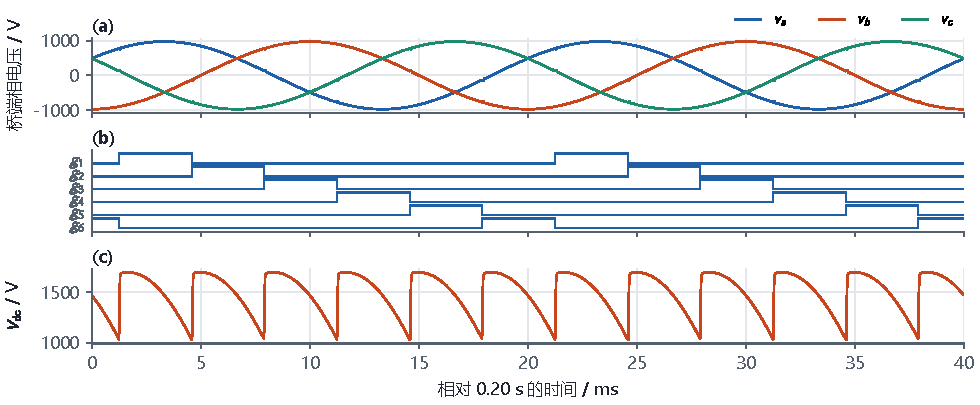
\includegraphics[width=\linewidth]{cs_detail}
\caption{六脉波详细模型 0.20--0.24~s 窗口：(a) 变压器二次侧相电压，(b) 六路门极，(c) 瞬时直流电压}
\label{fig:cs-detail}
\end{figure}
